\documentclass[a4paper,11pt]{article}
\input{/home/tof/Documents/Cozy/latex-include/preambule_lua.tex}
\newcommand{\showprof}{show them}  % comment this line if you don't want to see todo environment
\fancyhead[L]{Tutoriel Lycée Connecté}
\newdate{madate}{22}{09}{2020}
\fancyhead[R]{\displaydate{madate}} %\today
\fancyfoot[L]{~\\Christophe Viroulaud}
\fancyfoot[C]{\textbf{Page \thepage}}
\fancyfoot[R]{\includegraphics[width=2cm,align=t]{/home/tof/Documents/Cozy/latex-include/cc.png}}

\begin{document}
\begin{Form}
Le \emph{lycée connecté} est un outil très complet. Il propose de nombreux outils comparables à ceux d'un compte Google auxquels s'ajoutent des applications orientées éducation. Enfin il respecte la RGPD: les données sont stockées en France (prestataire OVH) et ne sont pas utilisées à des fins commerciales.
\section{Présentation}
\subsection{Page d'accueil}
La page d'accueil (figure \ref{accueil}) se découpe principalement en trois parties:
\begin{itemize}
\item le fil de nouveautés,
\item les widgets à gauche,
\item le bandeau de navigation en haut à droite.
\end{itemize}
\begin{figure}[!h]
\centering
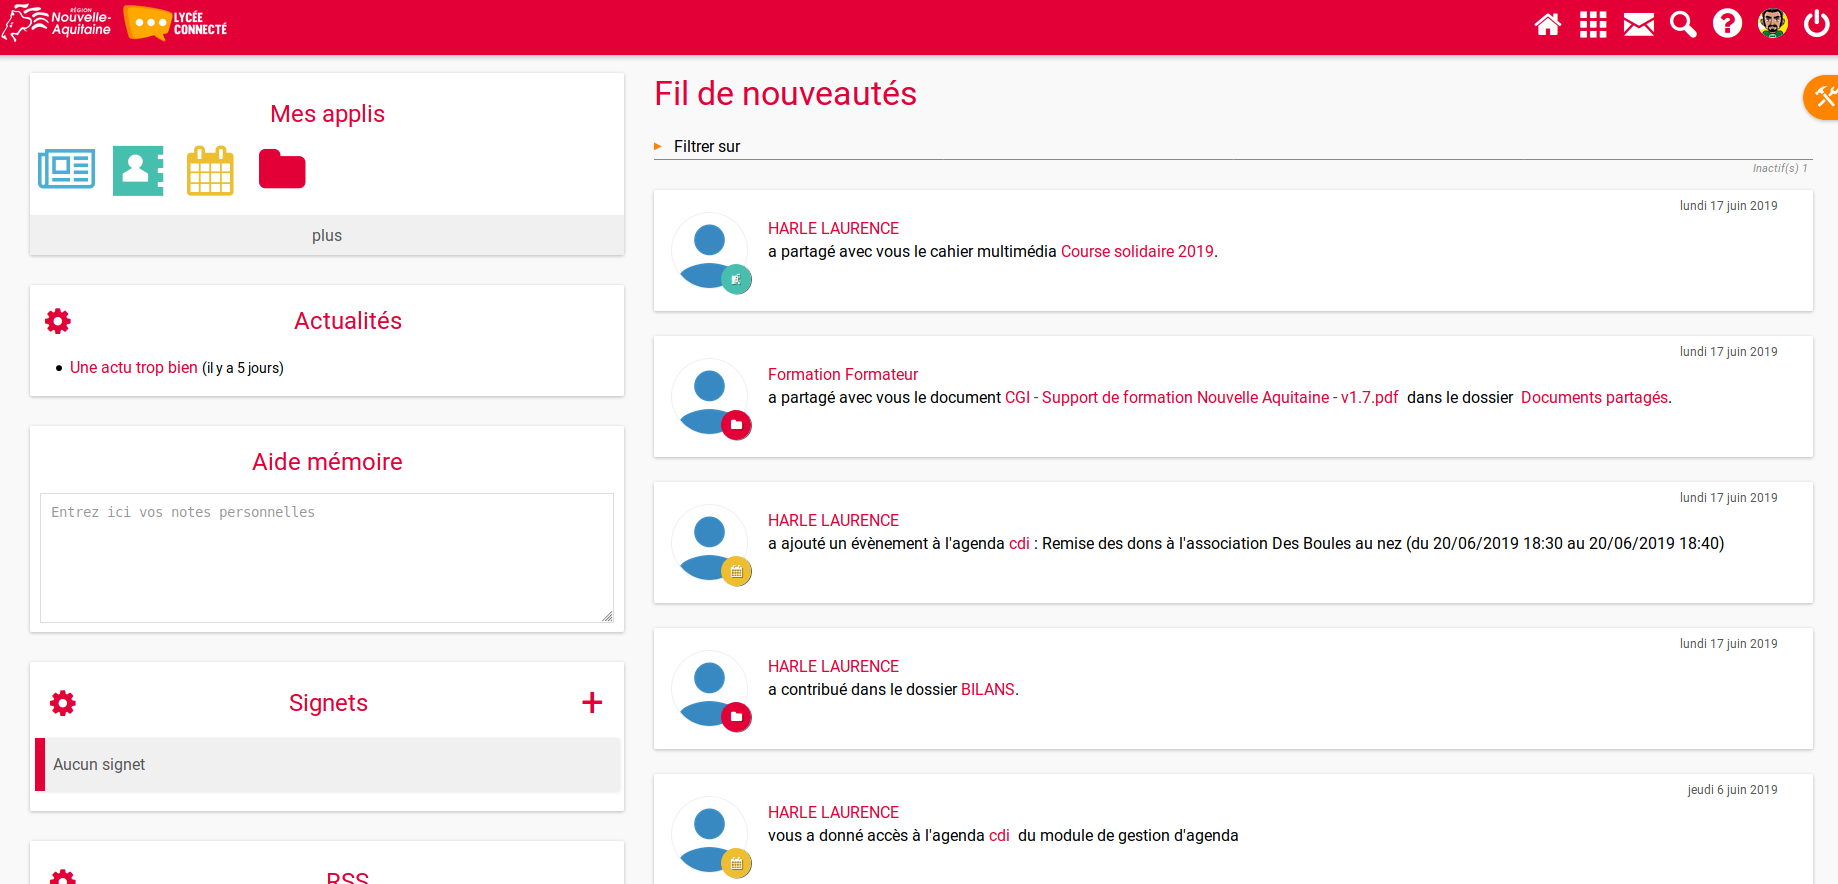
\includegraphics[width=13cm]{ressources/timeline.png}
\captionof{figure}{Page d'accueil}
\label{accueil}
\end{figure}
\subsection{Personnalisations}
\subsubsection{Fil de nouveautés}
Il affiche toutes les interactions vous concernant: partage de documents, envois de fichiers, commentaires.\\
Si certaines notifications ne vous intéressent pas, il faut cliquer sur \textbf{filtrer sur} et désélectionner les applications pour lesquelles vous ne voulez pas recevoir de notifications.
\subsubsection{Widgets}
Plusieurs widgets sont particulièrement intéressants:
\begin{itemize}
\item Signets: enregistrer un lien vers une page web.
\item Dictaphone: enregistrer rapidement du son (un microphone est nécessaire); le fichier est enregistré dans l'application \emph{Documents}. Nous reviendrons en détails sur cette application dans la section \ref{documents}.
\item Mes applis: raccourci vers les applications fréquemment utilisées. 
\end{itemize}
\begin{activite}
Il est possible de modifier la liste des applications favorites en procédant comme suit (figures \ref{appacces} et \ref{app}). Modifier les applications favorites.
\end{activite}
\begin{figure}[!h]
\centering
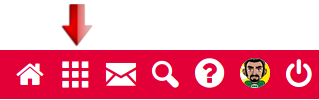
\includegraphics[width=5cm]{ressources/bandeauapp.png}
\captionof{figure}{Accéder aux applications}
\label{appacces}
\end{figure}
\begin{figure}[!h]
\centering
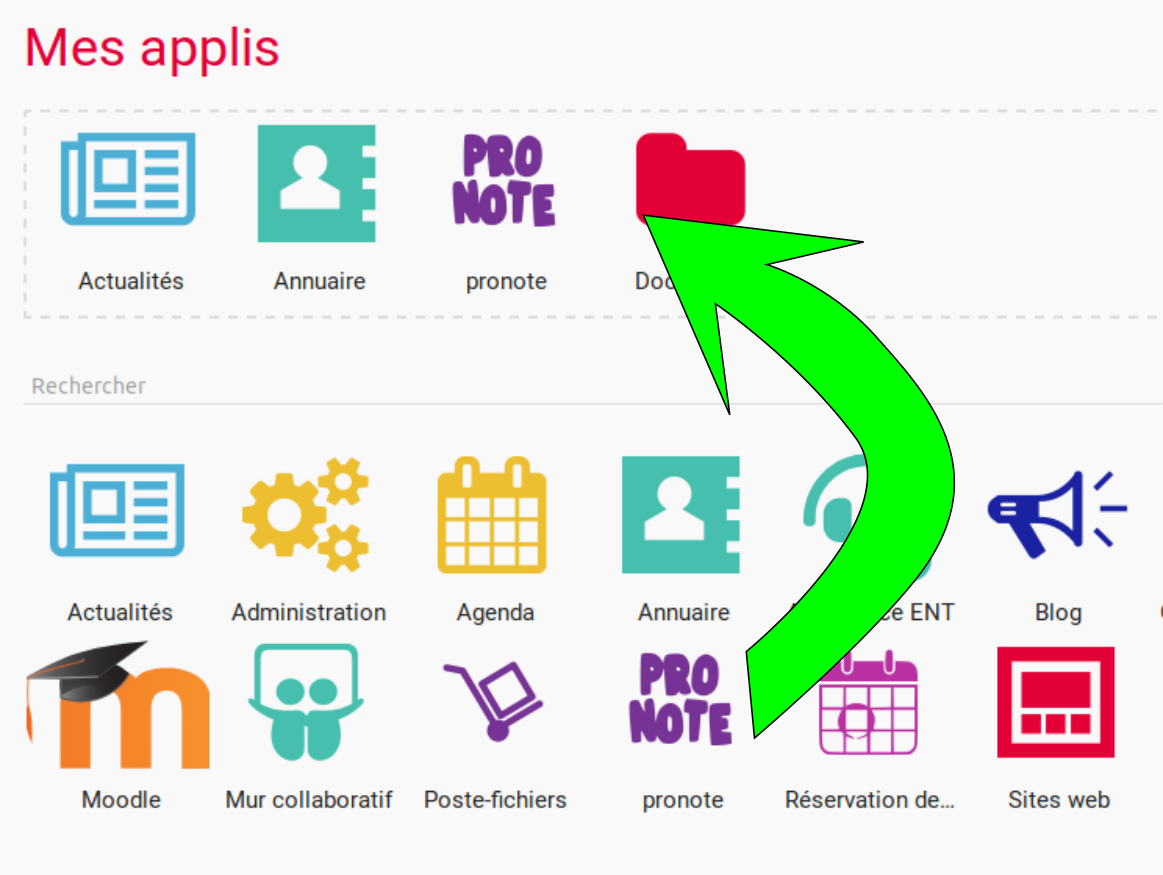
\includegraphics[width=10cm]{ressources/glisser.png}
\captionof{figure}{Ajouter une application au widget d'accueil}
\label{app}
\end{figure}
\section{Applications}
Toutes les applications sont des services libres qui existent déjà sur le web. Elles ont été adaptées (graphiquement, fonctionnalités de partage...) au \emph{Lycée Connecté} afin d'assurer un environnement cohérent.
\subsection{Partager}
Il s'agit du point important à maîtriser. Le principe du partage est le même dans toutes les applications (au moins la très grande majorité).\\
Testons ce comportement à travers l'application \emph{Carte mentale}. Nous pourrons l'appliquer ensuite aux autres applications.
\begin{figure}[!h]
\centering

\includegraphics[width=2cm]{ressources/mur.png}
\captionof{figure}{Mur collaboratif}
\label{mur}
\end{figure}
\begin{activite}
\begin{enumerate}
\item Ouvrir l'application \emph{Mur collaboratif}.
\item Créer un nouveau mur. Penser à enregistrer en bas à droite.
\item Tester les possibilités du mur collaboratif en cliquant ur \emph{Nouvelle note}.
\item Cliquer sur \emph{Mur collaboratif} pour revenir à la liste des murs.
\item Cliquer \textbf{une fois} sur le $\oplus$ (figure \ref{param-mur}) de l'étiquette représentant le mur. Un bandeau jaune apparaît en bas de l'écran (figure \ref{menubas}).
\item Choisir \textbf{Partager}. Une fenêtre apparaît: figure \ref{partage}.
\item Rechercher un nom de personne, groupe ou classe.
\item Attribuer les droits:
\begin{itemize}
\item Lecteur: pas de modification possible.
\item Contributeur: l'utilisateur peut ajouter des informations dans le mur.
\item Gestionnaire: l'utilisateur peut renommer voire supprimer le document.
\item Ne pas oublier de cliquer sur \emph{Partager} en haut à droite.
\end{itemize}
\end{enumerate}
\end{activite}
\begin{figure}[!h]
\centering
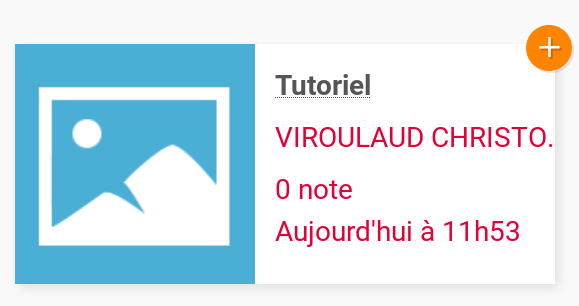
\includegraphics[width=4cm]{ressources/mur_parametre.png}
\captionof{figure}{Paramètres d'un mur}
\label{param-mur}
\end{figure}
\medskip
\begin{figure}[!h]
\centering

\includegraphics[width=10cm]{ressources/menubas.png}
\captionof{figure}{Menu de paramètres}
\label{menubas}
\end{figure}
\begin{figure}[!h]
\centering
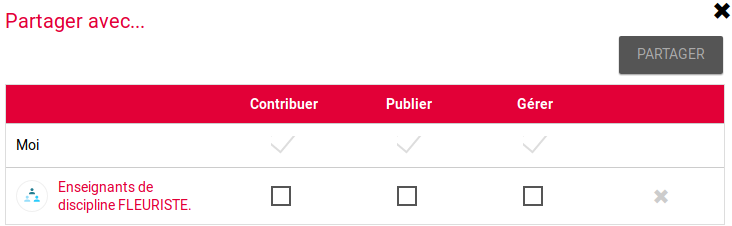
\includegraphics[width=7cm]{ressources/partage.png}
\captionof{figure}{Partage}
\label{partage}
\end{figure}
Les applications suivantes ont un fonctionnement très similaire à \emph{Mur collaboratif}:
\begin{center}
\begin{tabular}{cc}

\includegraphics[width=2cm]{ressources/carte.png}
 & 
\includegraphics[width=2cm]{ressources/frise.png}
 \\ 
Carte mentale & Frise chronologique \\ 
\end{tabular} 
\end{center}

\subsection{Documents}
Elle s'ouvre via l'icône:
\begin{figure}[!h]
\centering

\includegraphics[width=2cm]{ressources/documents.png}
\captionof{figure}{Documents}
\label{docs}
\end{figure}
\\C'est l'équivalent du \emph{Drive} de Google. Vous pouvez stocker tous types de documents (textes, images, pdf). En cliquant une fois sur un document le même bandeau jaune (figure \ref{menubas}) des paramètres apparaît en bas de page.\\
Dans le bandeau de gauche, trois sections sont présentées:
\begin{itemize}
\item Documents personnels: visibles uniquement par vous.
\item Documents partagés: ceux que vous partagez ou que d'autres vous ont partagé.
\item Documents ajoutés dans les applis: Nous retrouvons ici par exemple les sons enregistrés depuis le \emph{Dictaphone} de la page d'accueil.
\end{itemize}
\subsection{LibreOffice Online}
Depuis l'application \emph{Documents} il est possible de créer directement un document Texte, un Classeur ou un Diaporama. Mieux ce document peut être partagé et rédigé à plusieurs mains.
\begin{activite}
\begin{enumerate}
\item Dans \emph{Documents}, cliquer sur \textbf{Créer un document}.
\item Choisir \emph{Texte} et donner un nom au document.
\item Une nouvelle fenêtre apparaît. Les personnes familières de LibreOffice reconnaîtront les fonctionnalités du logiciel.
\item Revenir sur la page \emph{Documents}. Le fichier est présent dans l'onglet \emph{Documents personnels}.
\item Partager ce document avec les autres membres du groupe.
\item Écrire le document à plusieurs.
\end{enumerate}
\end{activite}
\subsection{Peertube}
C'est le Youtube pour l'Éducation Nationale.
\begin{figure}[!h]
\centering

\includegraphics[width=2cm]{ressources/peertube.png}
\captionof{figure}{Peertube}
\label{peertube}
\end{figure}
\\Le fonctionnement est un peu différent des applications précédentes. Il n'y a pas le principe du partage mais nous retrouvons le principe des listes de lecture de Youtube. Ce qu'il faut savoir faire:
\begin{itemize}
\item Créer une chaîne: depuis le menu de paramètres (les trois points verticaux de la figure \ref{param-peertube}), choisir \emph{paramètres des canaux}. Une chaîne par défaut existe; elle porte le nom de l'identifiant de l'utilisateur.
\end{itemize}
\begin{figure}[!h]
\centering

\includegraphics[width=5cm]{ressources/comptepeertube.png}
\captionof{figure}{Paramètres Peertube}
\label{param-peertube}
\end{figure}
\begin{itemize}
\item Importer une vidéo: Il suffit de cliquer sur le bouton en haut à droite (figure \ref{enligne}). Une fois la vidéo téléchargée, il suffira de choisir la chaîne de diffusion.
\end{itemize}
\begin{figure}[!h]
\centering

\includegraphics[width=5cm]{ressources/mettreenligne.png}
\captionof{figure}{Mettre une vidéo en ligne}
\label{enligne}
\end{figure}
\begin{itemize}
\item Rechercher une chaîne: Il faut donner le nom de sa chaîne aux élèves. Ils la chercheront depuis la barre de recherche en haut à droite. Il pourront également s'abonner à la chaîne.
\end{itemize}
\subsection{Blog}
Un blog est une suite d'articles qui peuvent contenir du texte et de nombreux contenus.
\begin{figure}[!h]
\centering

\includegraphics[width=2cm]{ressources/blog.png}
\captionof{figure}{Blog}
\label{blog}
\end{figure}
\\L'avantage ici est qu'il est possible d'insérer les documents du \emph{Lycée Connecté}, les vidéos \emph{Peertube}...
\begin{activite}
\begin{enumerate}
\item Créer un blog.
\item Le partager (en cliquant une fois) avec les autres membres du groupe.
\item Entrer dans le blog (en double-cliquant) et créer un article.
\item Insérer une vidéo \emph{Peertube} dans l'article.
\end{enumerate}
\end{activite}
\subsection{Exercices}
Cette application peut paraître un doublon du QCM de Pronote. Les fonctionnalités sont similaires. Elle a cependant l'avantage de profiter de l'univers cohérent du \emph{lycée connecté}. Il est par exemple possible d'insérer dans une question, un document (texte, audio, vidéo) déjà présent dans \emph{Documents}.
\begin{figure}[!h]
\centering

\includegraphics[width=2cm]{ressources/exercices.png}
\captionof{figure}{Exercices}
\label{exo}
\end{figure}
\begin{activite}
\begin{enumerate}
\item Créer un exercice.
\item Ajouter plusieurs questions et tester les différents modes de questionnement.
\item Insérer un document dans une question.
\item Visualiser le \emph{mode apprenant}.
\item Publier l'exercice. Le partager avec les autres membres du groupe. Régler les divers paramètres.
\end{enumerate}
\end{activite}

\subsection{Poste fichiers}
\begin{figure}[!h]
\centering

\includegraphics[width=2cm]{ressources/poste.png}
\captionof{figure}{Poste-fichiers}
\label{poste}
\end{figure}
Il peut être utile d'envoyer de gros fichiers qui ne peuvent loger dans un simple mail. L'application \emph{Poste-fichiers} permet de partager de gros documents (plusieurs Mo voire Go).

\section{Communiquer}
\subsection{Adresse mail}
Chaque utilisateur du \emph{lycée connecté} possède une adresse mail. Par défaut il s'agit de \emph{monidentifiant@lyceeconnecte.fr}. Pour vérifier la construction de l'adresse, il faut se rendre dans les paramètres du compte (figure \ref{compte}) et sélectionner ensuite l'onglet \emph{Messagerie} (figure \ref{comptemail}).
\begin{figure}[!h]
\centering
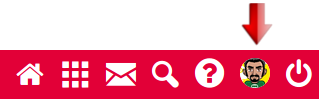
\includegraphics[width=5cm]{ressources/bandeaucompte.png}
\captionof{figure}{Paramètres du compte}
\label{compte}
\end{figure}
\begin{figure}[!h]
\centering
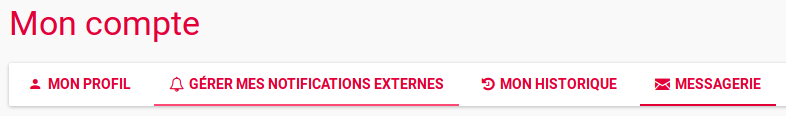
\includegraphics[width=10cm]{ressources/moncompte.png}
\captionof{figure}{Paramètres de messagerie}
\label{comptemail}
\end{figure}
\\L'adresse mail figure sur cette page. Il s'y trouve également les paramètres de configuration des clients de messagerie (Outlook, Thunderbird...). Cette adresse mail est similaire à n'importe quelle autre. Il est ainsi possible de l'utiliser à l'extérieur du \emph{lycée connecté}.\\
Nous accédons à la boîte de messagerie depuis l'icône ci- après:
\begin{figure}[!h]
\centering

\includegraphics[width=2cm]{ressources/mail.png}
\captionof{figure}{Boîte de réception}
\label{mail}
\end{figure}
\begin{activite}
\begin{enumerate}
\item Écrire un mail à \emph{christophe.viroulaud3@lyceeconnecte.fr}. Remarquer qu'il est possible d'envoyer un mail à toute une classe, un groupe...
\item Dans le mail, insérer un lien (figure \ref{lien1}) vers un \emph{mur collaboratif} ou une \emph{carte mentale} (figure \ref{lien2}) précédemment créée.
\end{enumerate}
\end{activite}
\begin{figure}[!h]
\centering
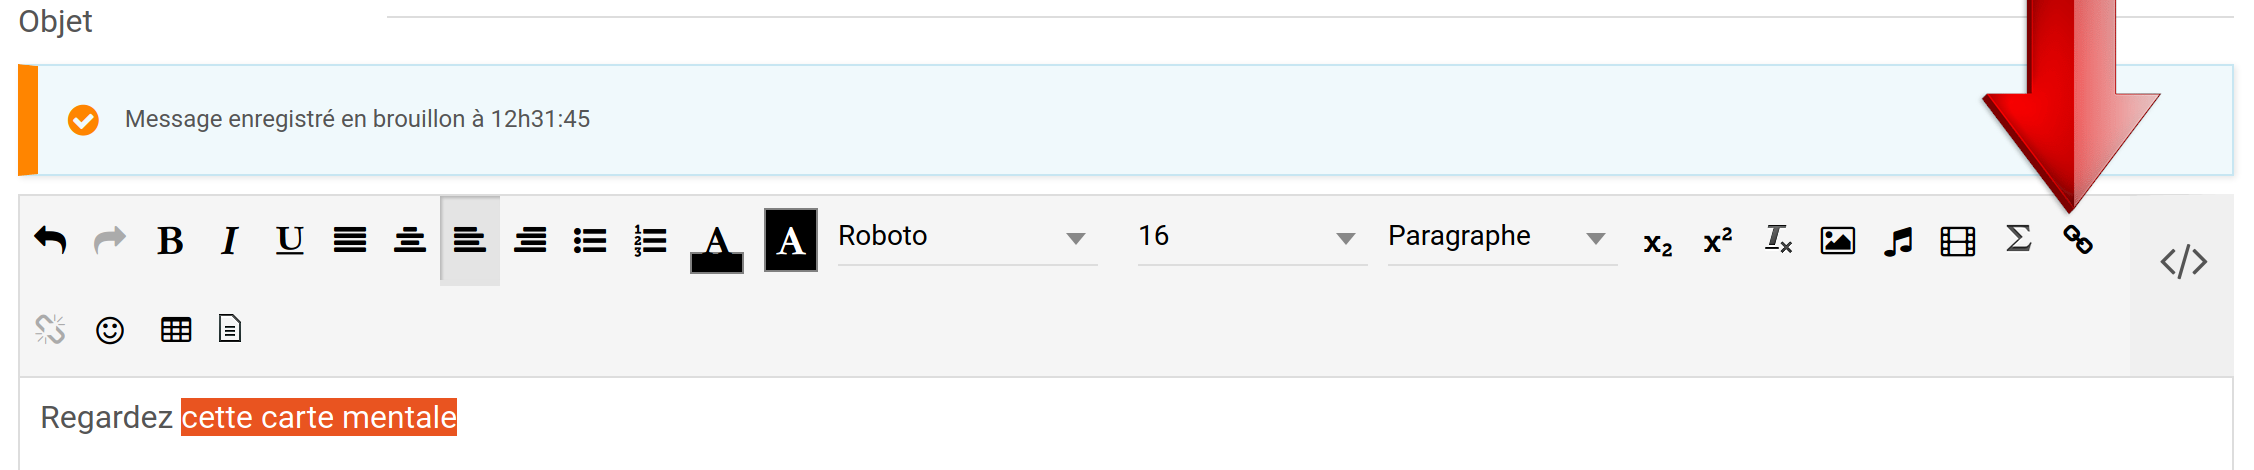
\includegraphics[width=7cm]{ressources/lienmail1.png}
\captionof{figure}{Insérer un lien}
\label{lien1}
\end{figure}
\begin{figure}[!h]
\centering
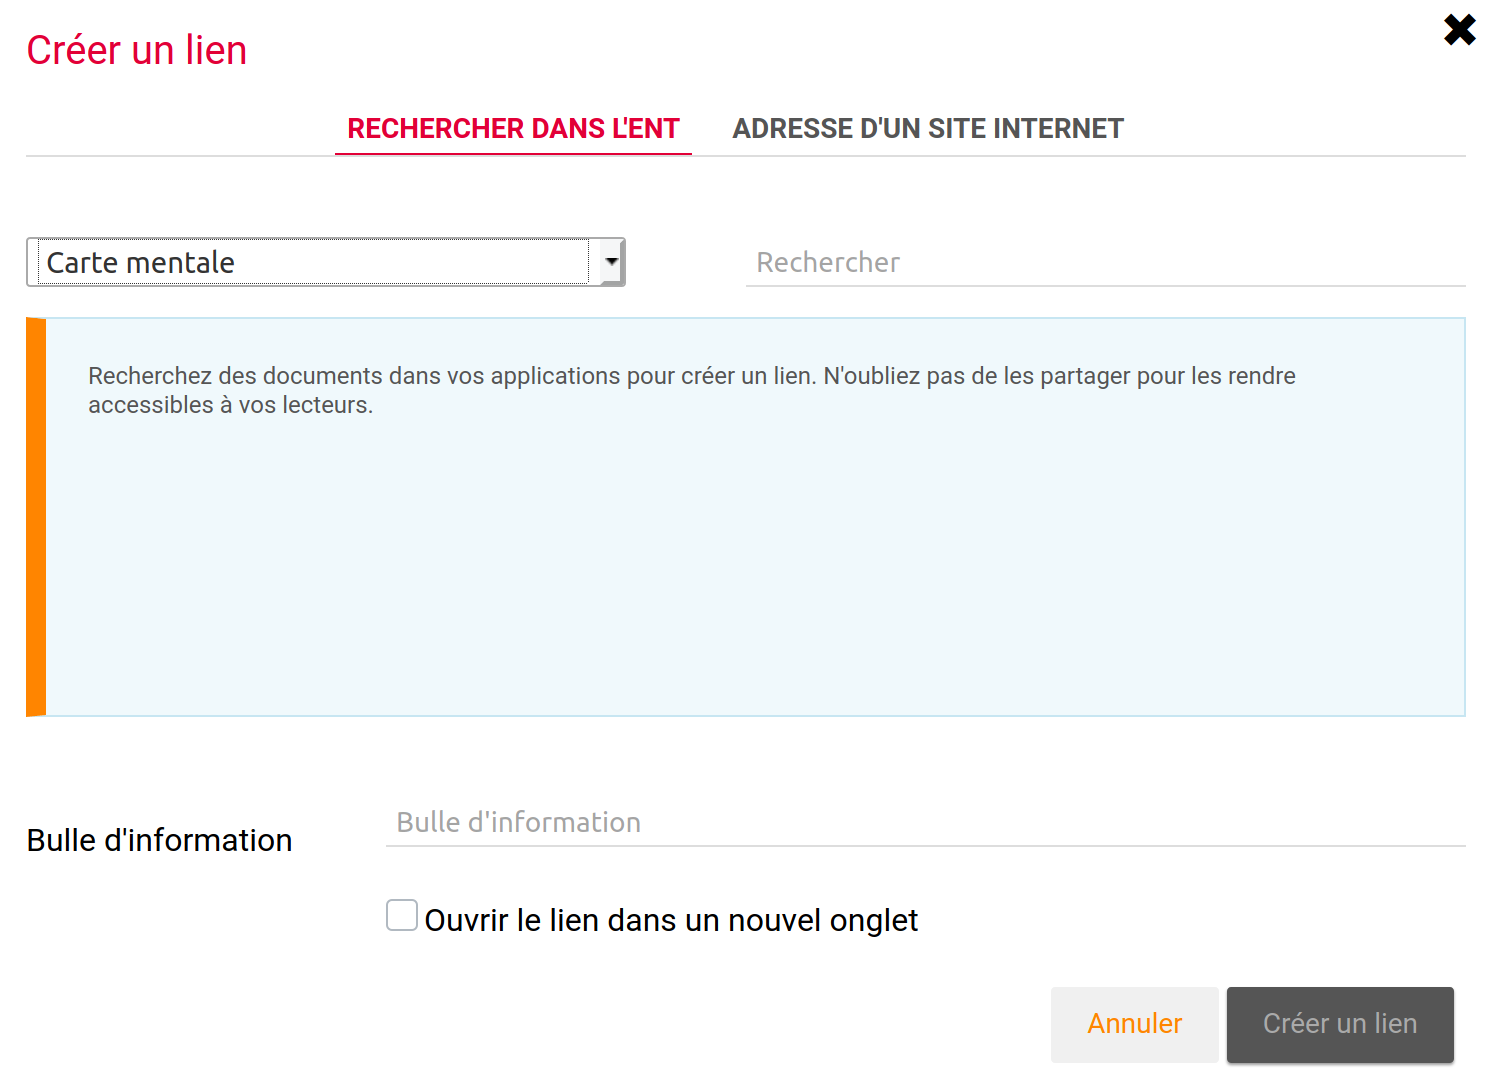
\includegraphics[width=6cm]{ressources/lienmail2.png}
\captionof{figure}{Insérer un objet}
\label{lien2}
\end{figure}
\subsection{Forum}
\begin{figure}[!h]
\centering

\includegraphics[width=2cm]{ressources/forum.png}
\captionof{figure}{Forum}
\label{forum}
\end{figure}
Il s'agit d'un forum classique comme nous pouvons en trouver de nombreux sur le web, mais amélioré des fonctionnalités du \emph{lycée connecté} (partage, ajout de documents...)
\subsection{Web-conférence}
\begin{figure}[!h]
\centering
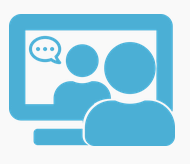
\includegraphics[width=2cm]{ressources/webconf.png}
\captionof{figure}{Web-conférence}
\label{webconf}
\end{figure}
C'est un outil similaire à la \emph{classe à la maison} du CNED. Il est possible de créer plusieurs salles puis de partager le lien de connexion (par mail par exemple) aux élèves.
Une fois dans la salle, plusieurs options sont proposées. Il est possible de charger une présentation externe, écrire à main levée, partager une vidéo... 
\subsection{Riot}
\begin{figure}[!h]
\centering

\includegraphics[width=2cm]{ressources/riot.png}
\captionof{figure}{Riot: messagerie instantanée}
\label{riot}
\end{figure}
C'est un outil de messagerie instantanée. Contrairement à \emph{Discord} ou autres, l'outil déployé sur le \emph{lycée connecté} respecte la RGPD.\\
Une fois entré dans l'application, il faut créer un salon ou en rejoindre un déjà existant.
\begin{activite}
\begin{enumerate}
\item Rejoindre le salon \emph{test-viroulaud}.
\item Créer un salon.
\item Modifier les paramètres de ce salon.
\end{enumerate}
\end{activite}
\end{Form}
\end{document}